% %%%%%%%%%%%%%%%%%%%%%%%%%%%%%%%%%%%%%%%%%%%%%%%%%%%%%%%%%%%%%%%%%%%%%%%%%%%%%%
%                           Making Mario Work Hard
% %%%%%%%%%%%%%%%%%%%%%%%%%%%%%%%%%%%%%%%%%%%%%%%%%%%%%%%%%%%%%%%%%%%%%%%%%%%%%%



% ------------------------------------------------------------------------------
% PACKAGES & DOCUMENT CONFIGURATION
% ------------------------------------------------------------------------------

\documentclass[11pt, a4paper, oneside]{report} % A4, 11pt font, one-sided
\usepackage[english]{babel}
\usepackage[utf8]{inputenc} %setlength{parskip}{0.7em}
\usepackage{bibentry}
\usepackage[margin= 1.3in]{geometry}
\usepackage[colorinlistoftodos]{todonotes}
\usepackage{epigraph}
\usepackage{graphicx}
\usepackage{listings}
\usepackage{xcolor}
% \usepackage{algorithm}
% \usepackage[noend]{algpseudocode}

\usepackage{url}
\usepackage[nottoc]{tocbibind}
 \usepackage{caption}

\lstset { %
    language=C++,
    backgroundcolor=\color{black!5}, % set backgroundcolor
    basicstyle=\footnotesize,% basic font setting
}

\definecolor{listinggray}{gray}{0.9}
\definecolor{lbcolor}{rgb}{0.9,0.9,0.9}
\lstset{
    backgroundcolor=\color{lbcolor},
    tabsize=4,    
%   rulecolor=,
    language=[GNU]C++,
        basicstyle=\scriptsize,
        % upquote=true,
        aboveskip={1.5\baselineskip},
        columns=fixed,
        showstringspaces=false,
        extendedchars=false,
        breaklines=true,
        prebreak = \raisebox{0ex}[0ex][0ex]{\ensuremath{\hookleftarrow}},
        frame=single,
        numbers=left,
        showtabs=false,
        showspaces=false,
        showstringspaces=false,
        identifierstyle=\ttfamily,
        keywordstyle=\color[rgb]{0,0,1},
        commentstyle=\color[rgb]{0.026,0.112,0.095},
        stringstyle=\color[rgb]{0.627,0.126,0.941},
        numberstyle=\color[rgb]{0.205, 0.142, 0.73},
%        \lstdefinestyle{C++}{language=C++,style=numbers}’.
}
\lstset{
    backgroundcolor=\color{lbcolor},
    tabsize=4,
  language=C++,
  captionpos=b,
  tabsize=3,
  frame=lines,
  numbers=left,
  numberstyle=\tiny,
  numbersep=5pt,
  breaklines=true,
  showstringspaces=false,
  basicstyle=\footnotesize,
%  identifierstyle=\color{magenta},
  keywordstyle=\color[rgb]{0,0,1},
  % commentstyle=\color{Darkgreen},
  stringstyle=\color{red}
  }

\definecolor{Gray}{gray}{0.70}
\definecolor{LightCyan}{rgb}{0.88,1,1}

% \newcolumntype{a}{>{\columncolor{Gray}}c}
% \newcolumntype{b}{>{\columncolor{white}}c}


\linespread{1.1}

\begin{document}

% ------------------------------------------------------------------------------
% TITLE PAGE
% ------------------------------------------------------------------------------

% \begin{titlepage}
%     \begin{center}
%         \vspace*{4cm}

%         \Huge\textbf{Making Mario Work Hard}

%         % \vspace{0.5cm}
%         % Thesis Subtitle

%         \vspace{2.5cm}

%        \Large\textbf{Aaron Ceross}
%        \\Supervisor: Dr. Benjamin Sach

%         % \vfill
%         \vspace{0.8cm}

%         MSc Thesis Project\\
%         COMSM3201 MSc Project, Computer Science

%         Research Review\\
%         COMSM2202 Research Skills

%         \vspace{0.8cm}

%         % \includegraphics[width=0.4\textwidth]{university}

%         % Department Name\\
%         % University Name\\
%         % Country\\
%         \today

%     \end{center}
% \end{titlepage}


% ------------------------------------------------------------------------------
% Executive Summary
% ------------------------------------------------------------------------------

\chapter*{Executive Summary}

Blank at the moment

% ------------------------------------------------------------------------------
% ACKNOWLEDGEMENTS
% ------------------------------------------------------------------------------

\chapter*{Acknowledgements}

While this thesis was the culmination and result of many long solitary hours of
research and development no effort is truly without support. I would like to
extend immense thanks and gratitude to Dr Benjamin Sach for his guidance and
support throughout the project. He has been an unrivalled source of information
and helping me find a deeper appreciation of computer science and mathematics.

I would also like especially thank my dear Tingting for being willing to
subjected to innumerable proof reads and generally being incredibly patient and
understanding throughout the project's development process. Without her
feedback, support, and encouragement, this project would not have been anywhere
near as successful as it has been.


% ------------------------------------------------------------------------------
% TABLE OF CONTENTS
% ------------------------------------------------------------------------------

\tableofcontents


% ------------------------------------------------------------------------------
% CHP 1 --- INTRODUCTION
% ------------------------------------------------------------------------------

\chapter{Aims and Objectives}

\epigraph{``The obvious objective of video games is to entertain people by
surprising them with new experiences.''}{Shigeru Miyamoto}

\section{Background, context, and motivation}

An NP-complete problem is one with a solution that can be \textit{verified}
quickly in polynomial time, though an existing solution is not readily known or
\textit{identifiable} \cite{cook1984can}. It has been proven that certain
classic video games, such as \textit{Super Mario Bros} \cite{Aloupis2012}, are
computationally hard in that the character could be made to solve an arbitrary
instance of a Boolean satisfiability problem (SAT). SAT is a type of NP-complete
problem in which the variables of the formula may be consistently replaced by
the values TRUE or FALSE in a way that the formula evaluates to TRUE, or
`satisfiable'.

The primary motivation of this research is to investigate the feasibility of
utilising the video game medium as an effective visualisation of computational
complexity. If successful, this type of visualisation could have a wide range of
effects, including use as teaching tool to new learners  approaching the
subject. 


There are several challanges that need to be addressed in order for this method
to be feasible.

\section{Research objectives}

% This project concerns the complexity of Mario which is known to be NP-
% Complete. To prove this it was shown that Mario could be forced to solve an
% (arbitrary) instance of the satisfying assignment problem (``SAT'') --- this
% is called a reduction. One computational problem is reducible to another
% problem if it is possible to efficiently solve the first one when provided
% with an efficient algorithm for solving the other. A problem in NP is
% determined to be NP complete if any problem in NP is reducible to it.The aim
% of this project is to implement a simple platform game and a level generator.
% The level generator should take an input to the SAT problem and convert it
% into a Mario level. The project should also include an AI player which can
% play these levels by choosing a suitable path using an existing SAT solver.

The aim of this project is to produce a game engine that is capable of
visualising and demonstrating concepts in computational complexity through the
evaluation of different instances of SAT.\@ The game engine would be able to
take an instance of SAT and generate a human-playable level that is
computationally hard. This level would then be able to be solved by a SAT
solver. The solution to the level would then be visualised on screen. In order
to fulfil this aim, the research project will implement a game engine through
achieving the following objectives: \\

\begin{enumerate}

  \item Develop a platform game in which the mechanics are NP-hard;
  \item Develop a level generator which converts an instance of SAT into a playable level;
  \item Develop a visualisation of the SAT solving these levels by choosing a suitable path;
  \item Evaluate level-generation and display of the SAT solver's decisions for
        efficiency and success against an established criteria or one developed
        during the project.

\end{enumerate}

% \section{Scope of the research review}

% As shown in the preceding section, the research being undertaken brings together
% a diversity of broad topic areas, which is challenging. Given the research aims
% and objectives described above, the scope of the research review is to
% understand the current state of research and development in the following areas:

% \begin{enumerate}

%   \item The principles and concepts of computational complexity which class a task or activity as
%   `difficult' or `hard'. This includes an assessment of the characteristics which define the
%   differing classes of complexity;

%   \item  The tests of computational complexity that prescribe the different classifications through
%   Boolean satisfiability. This includes how these tests may be applied to video games, with
%   particular focus on 2D platform games;

%   \item The generation of video game content in order to produce the problem instances as levels in
%   an accurate and efficient manner.

%   \item Assessing the means for implementing these divergent areas of research in order to produce a
%   bespoke game engine that realises the research aim.


% \end{enumerate}

% \section{Scope of the research review}

As shown in the preceding section, the research being undertaken brings together
a diversity of broad topic areas, which is challenging. Given the research aims
and objectives described above, the scope of the research review is to
understand the current state of research and development in the following areas:

\begin{enumerate}

  \item The principles and concepts of computational complexity which class a task or activity as
  `difficult' or `hard'. This includes an assessment of the characteristics which define the
  differing classes of complexity;

  \item  The tests of computational complexity that prescribe the different classifications through
  Boolean satisfiability. This includes how these tests may be applied to video games, with
  particular focus on 2D platform games;

  \item The generation of video game content in order to produce the problem instances as levels in
  an accurate and efficient manner.

  \item Assessing the means for implementing these divergent areas of research in order to produce a
  bespoke game engine that realises the research aim.


\end{enumerate}

As shown from the range of topics above, the areas being investigated are
expansive and multi-faceted. Therefore, this research review surveys those
elements most relevant for the implementation and development of the game engine
software.

\section{Thesis Structure}

This research project is divided between 66\% Type I (software development) and
34\% Type II (investigatory, research). The structure of this document reflects
this division in that the theoretical concepts are broadly introduced and
discussed insofar as relevant to the research aim. The discussion strongly
focuses on the  implementaiton and development challenges in realising these
concepts in the project.

Chapter 2 covers the fundamental concepts in computational complexity,
identifying which characteristics render a task difficult. The chapter discusses
the well-known P vs NP question and explains the NP-hardness complexity class.
Other classes which are later explored within the project are also demonstrated
and analysed.

The overview of computational complexity provides the basis for the discussion
in Chapter 3 on Boolean Satisfiability problems and SAT solving software. In
addition to explaining the major features of SAT solvers, the chapter also
identifies SAT solvers which had been considered during the project's
development.


%---------------------------------------------------------------------------------------------------
% CHP 2 --- COMPUTATIONAL COMPLEXITY AND VIDEO GAMES
%---------------------------------------------------------------------------------------------------

\chapter{Computational complexity theory}

\epigraph{``In general, it is much harder to \textit{find} a solution to a problem than to
\textit{recognize} one when it is presented''}{Stephen A Cook \cite{cook1984can}}

\section{Fundamental concepts}

\subsection{Definitions}

The goals of the research project are to visualise computational complexity
through video games. Therefore, the literature review begins with identifying
the relevant key concepts in computational complexity theory in order to
understand what characteristics makes a problem computationally hard.

Computational complexity theory is concerned with assessing and classifying the
difficulty of defined tasks as well as the relationship between such tasks.
Within computational complexity, there exist different types of problems, termed
\textit{complexity classes}. Complexity classes rank the difficulty of differing
types of problems. Of the many types of problems which can exist in
computational complexity theory, the two fundamental types this research project
is interested in are (\textit{i}) decision problems and (\textit{ii}) search
problems. The importance of the distinction between these two types will be made
clearer when discussing Boolean satisfiability (Chapter 2) and procedural
content generation (Chapter 5).

\subsubsection{Decision problems and search problems}

A decision problem is a binary choice one wherein, on an infinite set of inputs,
the question may be answered `\textit{yes}' or `\textit{no}'  It is common  to
define the decision problem equivalency as: ``the set of inputs for which the
problem returns \textit{yes}''. Most problems may be reduced to a decision
problem \cite{kendall2008survey}, which is important in that the determination
of whether a solution exists or not is required in order to solve the
complementary search problem \cite{Goldreich:2008}.

Search problems represent a significant area of research in computer science
(citation needed), covering topics such as sorting and identifying the shortest
path \cite{Goldreich:2008}. A search problem consists of the identification of a
solution from a set of solutions (possibly infinite or empty). Therefore, given
an instance of a search problem, a solution must be found or return a
determination that no solution exists in such instance.

%  More on Search and Decision problems

\subsubsection{The concept of reductions}

Different complexity classes may be defined through the ability to transform an
instance of one type of problem into another. This ic alled a reduction and is
the basis for classifying the 

The most common reduction is a polynomial time reduction which means - ////something ////



///// COPY PASTE FROM WIKI /////////////////////////////////////////////////////
Many complexity classes are defined using the concept of a reduction. A
reduction is a transformation of one problem into another problem. It captures
the informal notion of a problem being at least as difficult as another problem.
For instance, if a problem X can be solved using an algorithm for Y, X is no
more difficult than Y, and we say that X reduces to Y. There are many different
types of reductions. 

The most commonly used reduction is a polynomial-time reduction. This means that
the reduction process takes polynomial time. For example, the problem of
squaring an integer can be reduced to the problem of multiplying two integers.
This means an algorithm for multiplying two integers can be used to square an
integer. Indeed, this can be done by giving the same input to both inputs of the
multiplication algorithm. Thus we see that squaring is not more difficult than
multiplication, since squaring can be reduced to multiplication.

////////////////////////////////////////////////////////////////////////////////

\subsection{Survey of complexity classes}

\subsubsection{P and NP}

The two fundamental complexity classes relevant for this research project are
\textbf{P} and \textbf{NP}\@. The P (polynomial) class of problems contain those
decision problems that are often described as `easy' problems
\cite{kendall2008survey} as the time required to solve such problem has an
upper- bound that scales by a polynomial function of the input
\cite{sipser2012introduction}. The other complexity class, NP (non-deterministic
polynomial), relates to those problems that do not have an efficient way of
finding a solution but can have a solution verified in polynomial time
\cite{Goldreich:2008, Papadimitriou:2003:CC:1074100.1074233}.

%  More on P and NP
% Therefore:
% \\

% \centerline{T(\textit{n}) = O(\textit{n}$^k$)}

% Where \textit{T}


\subsubsection{P vs NP Problem}

The P vs NP problem refers to search problems to which there exists an efficient
algorithm that given a solution to a given instance determines whether or not
the solution is correct\cite{sipser2012introduction,Goldreich:2008,
kendall2008survey,du2011theory}.\footnote{This is also sometimes described as
the P vs NP Question in literature} Although any given solution to an NP-
complete problem can be verified quickly (in polynomial time), there is no known
efficient way to locate a solution in the first place. A distinguishing
characteristic of of NP- complete problems is that there is no known efficient
solution to them \cite{Goldreich:2008}. That is, the time required to solve the
problem using any currently known algorithm increases very quickly as the size
of the problem grows.

\begin{figure}[h!]

  \centering
    
\includegraphics[scale=0.45]{pnp}
  \caption{Euler diagram illustrating the relationship between P and NP \cite{esfahbod:euler}.}
  \label{Euler}
\end{figure}


Proving that P = NP or P $\neq$ NP is one of the most important open questions
in theoretical computer science and has been described as one of seven principal
unsolved problems in the field of mathematics \cite{devlin2002millennium}. The
implications of P = NP are far-reaching. If it were possible to demonstrate that
P = NP (i.e. all NP problems can be solved in polynomial time), then it would
then be possible to solve difficult problems in polynomial time (see
Figure~\ref{Euler}). For every problem that has an efficiently verifiable
solution, that same solution could also be efficiently identified. While the
problem is still being researched and open to debate, there is wide belief that
P $\neq$ NP is more likely than P = NP \cite{Gasarch:2012:GCS:2261417.2261434}.


% Search problems, for example, are not known to be solveable in polynomial time.


\subsubsection{NP-hard}

A problem is considered to be classed as \textbf{NP-hard} if the solution's
algorithm may be adapted to solve any problem in NP. By extension, this will
then include all problems in P, which are contained within NP. It should be
noted that not all NP-hard problems fall within NP nor are NP-hard problems
necessarily decidable problems
\cite{sipser2012introduction,Goldreich:2008,kendall2008survey,du2011theory}.

\subsubsection{NP-complete}

When a problem is classed as both NP and NP-hard is said to be \textbf{NP-
complete} and are considered to be the hardest problems in NP
\cite{sipser2012introduction,Goldreich:2008,kendall2008survey,du2011theory}. A
problem that is NP- complete can have every other problem in NP reducible to it
\cite{papadimitriou2003computational}. `Reduction' in this sense that there
exists an algorithm in P that change a problem into another instance
\cite{du2011theory}.

\subsubsection{PSPACE}

Another relevant complexity class to this research review is \textbf{PSPACE}, as
some games have been proven to be in this class \cite{DBLP:conf/fun/Forisek10,
demaine2002push}.\footnote{Please refer to Chapter 3 of this research review for
further information.} PSPACE refers to decision problem which may be solved with
an amount of space polynomial in the size to its input
\cite{sipser2012introduction}. 

\subsubsection{EXSPACE}


\section{Chapter summary}

This chapter has identified the relevant complexity classes and problems in
order to establish that video games are computationally complex in Chapter 4. In
the next chapter, these concepts will be used to show how problem instances may
be proven to be NP-complete through the use of Boolean expressions. This will
provide the foundation for being able to develop a game engine which produces
computational hard levels in a video game.


%---------------------------------------------------------------------------------------------------
% CHP 3 --- BOOLEAN SAT SOLVERS
%---------------------------------------------------------------------------------------------------

\chapter{Boolean satisfiability problems}

\epigraph{``It is not of the essence of mathematics to be conversant with the
ideas of number and quantity.''}{George Boole}

Boolean satisfiability problesm (or SATs) serve as the basis for proving the
hardness of video games and have implications for the game engine design as well
as the design of the  game level (see chapters X and Y). 

% These game instanceswill then be completed by SAT solvers (specialised programs
% that solve instances of SAT) will be used to run tests through the constructed
% game.

\section{Principle concepts and definitions}

A Boolean formula is a logic expression with variables that have a value of
either TRUE or FALSE. These formulae also contain logical connectives, which
subscribe to an order of precedence: negation ($\neg$), conjunction($\wedge$),
disjunction ($\vee$), implication ($\leftarrow$), and equivalence
($\leftrightarrow$) \cite{balyo2010solving,gomes2008satisfiability}.

Formulae are constructed through literals, which is a variable (e.g. \textit{x}
or \textit{y}) or its complement (e.g. \textit{x} or $\neg$\textit{x}). Literals
are joined together in groups called clauses. The literals and clauses may be
joined either disjunctively (i.e. or conjunctively (i.e. the expressions must
collectively evaluate to true)

Of these constructions, the conjunctive normal form (CNF) is of particular
importance, especially in relation to finding solutions to satisfiability
problems, particularly those solving methods based on DPLL algorithm
\cite{gomes2008satisfiability} (See Section X below for further discussion). To
be in CNF, a formula must a conjunction of clauses, wherein those clauses are a
disjunctive of literals. The example below illustrates conjunctive normal form
with three clauses (joined together by $\wedge$ (AND)) containing three literals
(x, y, z).

\centerline{(x $\vee$ $\neg$y) $\wedge$ ($\neg$x $\vee$ z $\vee$ y) $\wedge$ ($\neg$z $\vee$ x)}

\par  \noindent To satisfy this expression, each clause must evaluate to TRUE as
they are conjunctively joined. If any clause were to be FALSE, the formula
twould be unsatisfiable.

\section{Boolean Satisfiability problem and NP-completeness}

The Boolean satisfiability problem (SAT) is the problem of determining if there
exists an assignment that satisfies a given Boolean formula. In order for such
assignment to be \textit{satisfiable}, the variables' values are replaced
constantly with TRUE or FALSE until the formula evaluates to TRUE. Where no such
assignment is possible (i.e. the formula evaluates to FALSE in all
combinations), the formula is determined to be \textit{unsatisfiable}
\cite{balyo2010solving,gomes2008satisfiability}. Therefore, given a CNF formula
\textit{F}, SAT may be posed as: does \textit{F} have a satisfying assignment?

This question has an important place in computer science as it was the first
problem proven to be NP-complete \cite{cook1971complexity}.\footnote{While this
is often described as \textit{Cook's Theorem} it had been independently verified
in \cite{levin1973universal} and is more accurately termed the \textit{Cook-
Levin Theorem}} In solving a SAT problem, the question involves not only
providing a yes or no, but also in finding an actual solution to the assignment
\cite{zhang2002quest}. Specialised software, SAT solvers (discussed in Section
3.2.2 below), provide these solutions, if one exists.

\subsection{Examples of SAT reductions}

Three-satisfiability or 3SAT is the SAT reduction is most relevant for the
research project as it has been used to demonstrate the NP- completeness of 2D
platform games  \cite{Aloupis2012}. In 3SAT, there may only ever be three
literals in each clause and at least of of the literals contain a value of TRUE
in order to achieve satisfiability \cite{balyo2010solving}.There is a variant of
the 3SAT, exactly 1-3-satisfiability or 1-in-3SAT above reduction wherein the
each clause must contain \textit{exactly} one literal \cite{balyo2010solving,
du2011theory}.

\section{Solving SAT instances}

SAT instances can be solved through a specialised piece of software called a SAT
solver.  Given a SAT instance, a SAT solver can either find a solution, which
would be a satisfying variable assignment or prove that no solution exists
\cite{zhang2002quest}. There are also stochastic methods based on local search
may be able to find satisfiable instances in a fast manner but are unable to
prove that an instance is in fact unsatisfiable \cite{gomes2008satisfiability}.
Understanding SAT solvers is fundamental to the development of the project's
game engine.

\subsection{Overview of the mechanics of SAT Solvers}

SAT solvers work recursively. SAT solvers features and functions.


\subsubsection{The DPLL algorithm}

The Davis-Putnam-Logemann-Loveland (DPLL) algorithm \cite{davis1962machine} is a
complete, systematic search algorithm which is based on backtracking. 

////BACKTRACKING IS WHAT???

The DPLL algorithm (see Figure~\ref{DPLL}) is able to decide the satisfiability
of a CNF SAT reduction as well as identify the satisfying assignment. It can
also show that a given Boolean formula is unsatisfiable. The algorithm achieves
these results through the use of branching and where clauses are found to be
FALSE, removes these from its search space.

\begin{figure}[h!]

  \centering
    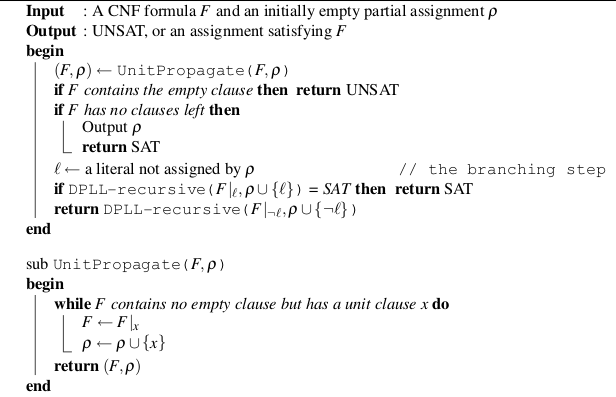
\includegraphics[scale=0.47]{dpll}
  \caption{DPLL in pseudo-code. Adapted from \cite{balyo2010solving,gomes2008satisfiability}.}
  \label{DPLL}
\end{figure}

The DPLL algorithm works with the CNF of a propositional logic expression (as
described in Section 3.1 above). Given that any formula may be converted into
CNF through the addition of new variables corresponding to the sub-formulae
\cite{tseitin1983complexity,Goldreich:2008}, DPLL may used to in all cases.


\subsubsection{Features of modern DPLL-based SAT solvers}

Modern DPPL-based SAT solvers are readily available and useful for this project.
There are currently a number of highly scalable SAT solvers, all based on the
classic DPLL search framework. These solvers, now also known as conflict-driven
clause learning (CDCL) solvers, can generally handle problem instances with
several million variables and clauses \cite{katebi2011empirical}. In the section
below, a collection of important features have been identified and have
relevance for the research project.

\begin{enumerate}


  \item \textbf{Selection heuristic} : \indent Also termed the `decision
strategy', this is the procedure of \textit{how} variables are selected and
assigned values. This aspect varies the most between different solvers can
significantly impact the efficiency of a solver
\cite{marques1999impact,gomes2008satisfiability, zhang2002quest}. There are a
range of strategies that can be employed including: Maximum occurrence in
clauses of minimum size heuristic \cite{jeroslow1990solving}, Bohm's heuristic
\cite{marques1999impact}, dynamic largest individual sum heuristic
\cite{marques1999grasp}, variable state independent decaying sum
\cite{moskewicz2001chaff}.

  % \subitem \textbf{Maximum occurance in clauses of minimum size heauristic} \cite{jeroslow1990solving}
  % \subitem \textbf{Bohm's heuristic} \cite{marques1999impact}
  % \subitem \textbf{Dynamic largest individual sum heauristic} \cite{marques1999grasp}
  % \subitem \textbf{Variable state independent decaying sum} \cite{moskewicz2001chaff}

%%%%%%%%%%%
%  is one of the features that vary the most from one
% SAT solver to another. Also referred to as the decision strategy, it can have a significant impact
% on the efficiency of the solver (see e.g. [160] for a survey).

% is one of the features that vary the most
% from one SAT solver to another. Also referred to as the decision strategy, it can have
% a significant impact on the efficiency of the solver (see e.g. [160] for a survey). The
% commonly employed strategies vary from randomly fixing literals to maximizing a
% moderately complex function of the current variable- and clause-state, such as the


%  MOMS (Maximum Occurrence in clauses
% of Minimum Size) heuristic [121] or the BOHM heuristic [cf. 32].

%One could select and fix the literal occurring most frequently in the yet unsatisfied clauses (the DLIS (Dynamic Largest
% Individual Sum) heuristic [161]), or choose a literal based on its weight which periodically decays
% but is boosted if a clause in which it appears is used in deriving a conflict, like in the VSIDS
% (Variable State Independent Decaying Sum) heuristic [170].

% Newer solvers like BerkMin \cite{Goldberg20071549}, , and RSat [184] employ
% further variations on this theme.

  \item \textbf{Clause learning} :  This method allows the solver to learn the
causes of unsatisfiability (sometimes termed `conflict') in clauses, using this
information to minimise the search space \cite{biere2009conflict}. When a
conflicting clause is encountered, the solver will needs try  to identify the
cause of a conflict and attempt to resolve it. This is achieved by asserting
that a solution does not exist in the particular search space, backtrack
(undoing the previous decisions) and continuing the search in a new one.
\cite{zhang2002quest}. This feature has been identified as one that improves the
underlying DPLL algorithm \cite{zhang2002quest,gomes2008satisfiability}.

  \item \textbf{Conflict clause minimization} Een and Sorensson
\cite{sorensson2005minisat} had first explored the use of this method in their
\texttt{MiniSat} solver. By utilising subsumption resolution, the size of the
learned conflict is minimised through the removal of literals that are implied
to be FALSE when the rest of the literals in the clause are FALSE
\cite{zhang2002quest}. This increased efficiency come with an increased
computational cost \cite{gomes2008satisfiability}.

  \item \textbf{Conflict-directed backjumping} : \indent Stallman and Sussman
\cite{stallman1977forward}   proposed a method to allow a solver to backtrack
directly to a decision-point \textit{p} if the variables at level \textit{p} or
lower are causing conflict. The assumption is therefore that there is no
solution to be found in this search space. It is agreed that this provides
greater efficiency and completeness to the procedure
\cite{gomes2008satisfiability}.


  \item \textbf{Fast backjumping} : Gomes \textit{et al}.
\cite{gomes2008satisfiability} describe this feature as allowing for a solver to
directly go to a lower decision level if even one branch in the search space is
in conflict. The authors note that this may not always increase efficiency
however. The branch at depth level \textit{d} is not marked as unsatisfiable but
rather a new variable and value is selected for that level, continuing with a
new clause. There has been some experimental work that suggests an increase in
solving efficiency \cite{gomes2008satisfiability, kottler2010sat}.

  \item \textbf{Watched literals scheme}:  This feature monitors two classes of
literals in an unsatisfied clause: TRUE or unassigned \cite{moskewicz2001chaff}.
As an empty clause will cause the DPLL to stop, This feature had been introduced
in the the \texttt{zChaff} solver and is utilised by many other solvers due to
the efficiency of the constraint propagation \cite{gomes2008satisfiability}.
This somewhat of an advancement of the `lazy data structures' which had been
introduced by the \texttt{Sato} solver \cite{zhang1997sato}. This feature has
furthered development of clause learning
\cite{zhang2002quest,gomes2008satisfiability}.

  \item \textbf{Assignment stack shrinking} : In the \texttt{Jerusat} SAT solver
\cite{nadel2002jerusat}, Nadel had introduced this feature which is based on
conflict clauses. Assignment stack shrinking servers to make the search area
more local by `shrinking' the conflict clause once it reaches a set threshold
\cite{Nadel:2010:ASS:2164073.2164111}. The `shrinking' is achieved by finding
the lowest decision level that is less than the immediate higher level by at 2.
The solver will then backtrack to this level and where possible, sets unassigned
literals of the clause to FALSE \cite{Nadel:2010:ASS:2164073.2164111}.

  \item \textbf{Randomised restarts} : This provides that the clause learning
algorithm can restart the branching process from decision level 0 while
retaining all the learned clauses \textit{et   al}. \cite{gomes1998boosting}.
Pioneered \texttt{zChaff} \cite{moskewicz2001chaff} many modern   SAT solvers
utilise highly aggressive restarts strategies, even below 20 backtracks, as it
demonstrably lowers the solution time \cite{gomes2008satisfiability}.

\end{enumerate}


\subsection{Converting a formula for SAT Solver Input}

The SAT instance must be read by the SAT solver. The standard input into a SAT
solver is a DIMACS CNF file\cite{DimacsSatFormat}. The file has a specified
format which allows the a formula to be input into the solver. Consider the
following example:



% % \footnote{DIMACS is % the
% Center for Discrete Mathematics and Theoretical Computer Science, a %
% collaborative effort between the Rutgers and Princeton Universities and research
% % laboratories from industry such as telecommunications giant AT&T}
                      \begin{lstlisting}

                        c example.cnf
                        c
                        p cnf 3 3
                         1  2 -3 0
                        -2  3  1 0
                        -1 -2  3 0
                      \end{lstlisting}

The \texttt{c} character is a comment indicator and will not be read by the SAT
solver. The SAT solver begins reading from the \texttt{p} character, which
indicates the problem line. On this line the SAT solver is given information
about the instance such as the format, in this case CNF, and the variables.   {}
and the clauses (). th. The reader ends a the `0' and begins reading the next
line until the end of file.

There are other formats available in a DIMACS satisfiability file, which include
the \texttt{sat} indicator instead of CNF\cite{DimacsSatFormat}. These other
formats were not explored during this project as the CNF format fulfilled the
project specification and was able to be rapidly deployed.

The DIMACS file requires that the clause only contain one literal of a variable
per clause \cite{DimacsSatFormat}. This means that x and not x are unable to
appear in the same clause. Attempting to create and run a file with this
structure will generate an error or an incorrect assessment of the SAT instance.


\section{Chapter summary}

Boolean satisfiability is the foundation for proving NP-hardness and NP-
completeness for the project, as will be demonstrated in the next chapter. The
availability of SAT solvers is also useful in order to try and test different
ones with the research project's game engine. Currently in the available
literature, there is very little research in this regard to the subject of
linking SAT solvers and video game engines, therefore representing a fertile
ground for development with this research project. The issue may be that these
solvers will not scale well with the game engine. In that respect, Brummayer et
al. \cite{brummayer2010automated} developed `fuzz testing' techniques which
allow for debugging errors in larger SAT instances. These techniques are useful
in ensuring the scalability of the SAT solver when attempting to solve large
levels.


% ------------------------------------------------------------------------------
% CHP 3 --- Computational complexity and video games
% ------------------------------------------------------------------------------

\chapter{Computational complexity and the hardness of (video) games}

\epigraph{``I strongly approve the study of games of reason, not for their own
sake, but because they help to perfect the art of thinking.''}{Gottfried
Wilhelm Leibniz}

\section{Overview}

Having established the concepts and means of testing for certain classes of
computational complexity in the previous chapters, this chapter will address the
assessment of complexity in video games. There is a growth of interest and
research in analysing `mainstream' video games, including two- dimensional (2D)
platform games  \cite{viglietta2014gaming, DBLP:conf/fun/Forisek10, Aloupis2012,
Smith:2008:FAP:1401843.1401858}. This chapter will identify the characteristics
and tests required to class a game as computationally hard. This will inform the
design considerations of the research project in Chapter 6.

Puzzles and games have long been a subject of complexity research with many
games being found to be at least within NP-hard \cite{kendall2008survey}. This
is often based on the assumption that P $\neq$ NP \cite{demaine2001playing}. The
list includes a variety of grid and block placement games, wherein a player
manoeuvres a block around a map to a specified location, such as
\textit{Minesweeper}\cite{kaye2000minesweeper} and
\textit{Tetris}\cite{demaine2003tetris}. Titles such as \textit{Sokoban},
\textit{Push} and \textit{PushPush}, which have been shown to be not only NP-
hard \cite{demaine2000pushpush}, but also PSPACE-hard
\cite{culberson1999sokoban, dor1999sokoban}. In the case of \textit{PushPush},
there have been proofs of NP-hardness not only in 2D but in 3D as well
\cite{o1999pushpush}. More recently, Gual\`{a} \textit{et al}. have demonstrated
that a number of `match-three' games, grid-based games which are popular on
mobile devices, such as \textit{Candy Crush Saga} and \textit{Bejewled} are NP-
hard \cite{DBLP:journals/corr/GualaLN14}.

The current trend in this field has been to assess classic franchises such as
\textit{Prince of Persia}, and \textit{Donkey Kong Country}. These studies are
more relevant to the research project as visualisation will utilise a 2D
platfomer resembling a game like \textit{Super Mario Bros}.


\section{2D platform games}

The research project focuses on developing a two-dimensional (2D) platform game
and thus the proof for NP-completeness is of particular interest. These games
are (very often) single-player games wherein the player traverses levels in
order to proceed to the next level. A `level' is a virtual spaces in which the
player character can manoeuvre and interact \cite{Burgun:2012}. The player's
game-play is influenced by the physics of the world, which often mean a
limitation of jump height and distance \cite{Burgun:2012}.

\subsubsection{Characteristics of 2D games}

In an examination of 2D platform games, Fori\v{s}ek provides an indicative list of
common puzzle elements found within the genre
\cite{Smith:2008:FAP:1401843.1401858,DBLP:conf/fun/Forisek10}. These include:

\begin{itemize}

  \item \textbf{long fall}: the maximum height from which the player character may fall without
                            receiving damage.

  \item \textbf{door opening}: the game world may include a variable number of doors and
                               suitable mechanisms to open them

  \item \textbf{door closing}: the game world contains a mechanism to close doors and a way for the
                               player to trigger the mechanisms

  \item \textbf{collecting items}: a set of items the player collects as part of the game. These may
                                   be necessary or optional content.

  \item \textbf{enemies}: Navigating the level may be made more challenging by having `enemy'
                          characters that must either be avoided or defeated by the player

\end{itemize}

\subsection{Characteristics of NP-hard games}

These above elements can be modeled into Boolean satisfiability problems, which
are known to NP-complete \cite{DBLP:conf/fun/Forisek10, cook1971complexity}.
The proofs of video games rely on this analogy and if a proof then removes
certain game elements, it is expected that the complexity of that game is
reduced \cite{viglietta2014gaming}.

Viglietta \cite{viglietta2014gaming} surveyed several classic video games games
published between 1980 and 1998, identifying general common elements and schemes
in video games that class them as computationally hard. These include
collectable items, activation of pathways (e.g.by key or button) by, or the
ability to destroy paths. Fori\v{s}ek \@\cite{DBLP:conf/fun/Forisek10} further
identifies several features specific to 2D platform video games which provide
for complexity, with particular focus on \textit{Prince of Persia}. In the work,
he posits a number of meta theorem, of which four are particularly relevant for
the research project:

\begin{itemize}

  \item \textbf{Meta-theorem 1}: A 2D platform game where the levels are constant and there is no
                                time limit is in P, even if the collecting items feature is present.

  \item \textbf{Meta-theorem 2}: A 2D platform game where the collecting items feature is present
                                 and a time limit is present as part of the instance is NP-hard.

  \item \textbf{Meta-theorem 3}: Any 2D platform game that exhibits the features long fall and
                                 opening doors is NP-hard.

  \item \textbf{Meta-theorem 4}: Any 2D platform game that exhibits the features long fall, opening
                                 doors and closing doors is PSPACE-hard.

\end{itemize}


Following the criteria above, it can be demonstrated that many platform games
are not only able to be classified as NP-hard but even PSPACE-hard in some
cases.

Aloupis \textit{et al} \cite{Aloupis2012} surveyed the complexity of classic
Nintendo franchises by considering that the games are essentially a decision
problem of reachability: ``given a level, is it possible to reach the goal point
\textit{t} from the start point \textit{s}''? The authors also review subsequent
\textit{Super Mario Bros} titles as well as other platform games such as
\textit{Donkey Kong Country}.

In the work, the authors had generalised the map size and left all other
elements of the game in the original settings. The proofs in \cite{Aloupis2012}
rely on a reduction of the game to 3SAT and the `level' was modelled to the
problem instance. This represents two potential points of difference from the
current research project. First, the research goal is to develop a means to
generate large levels and scale accordingly. Secondly, further reductions aside
from 3SAT may be explored.  \\

\begin{figure}[h!]

  \centering
    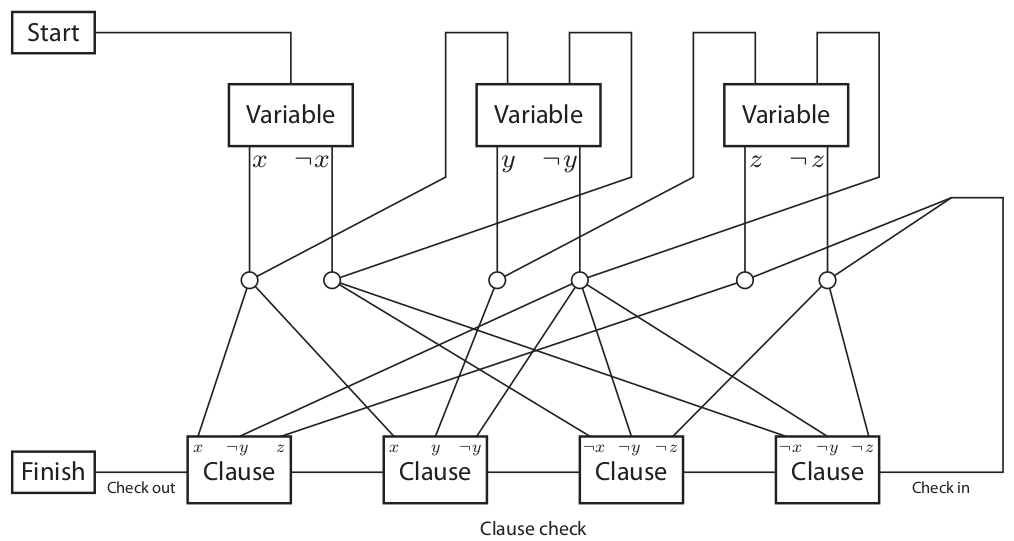
\includegraphics[scale=0.35]{aloupis_nphardness}
  \caption{Framework for NP-hardness \cite{Aloupis2012}.}
  \label{NP_hard}
\end{figure}

The framework for proving NP-hardness of games (see Figure~\ref{NP_hard}) is
reduced from 3SAT (described in Section 3.2.1 of this review). The player begins
the level at the \texttt{START} gadget and then traverses through variable
gadgets. A \textit{variable gadget} requires the player to make an choice, which
amounts to TRUE (\textit{x}) or FALSE (\( \neg \)\textit{x}) for the values in
the formula. These decisions allows the player to follow paths leading to
\textit{clause gadgets}. A clause gadget creates a permanent state change and as
a consequence, the player cannot access other paths connecting to that gadget.
As can be seen in the framework above, there are several areas of potential
crossover. To prevent such occurrence, \textit{crossover gadgets} prevent a
player from switching paths.

Once the player has passed through all the variable gadgets, the player can
proceed to the \texttt{FINISH} through a clause check path. This can only be
successfully traversed only if every clause gadget has been unlocked.




% \subsection{Proving a platformer is PSPACE-hard}

% % \subsubsection{\textit{Super Mario Bros}}

% % The construction of the games requires that that player character begins in a \texttt{Start} gadget
% % wherein the state requirement can be satisfied. In the case of \textit{Super Mario Bros}, the
% % \texttt{Start} gadget is a `Super Mushroom' that allows Mario to be in a large state, which is
% % necessary to reach the \texttt{Finish} gadget.

% \subsubsection{\textit{Donkey Kong Country}}

\section{Chapter summary}

The frameworks provided by \cite{Aloupis2012} give a comprehensive model for the
project's implementation. Modelling these gadgets to SAT clauses will form a
significant area of the research project's work. By utilising the metatheorms
provided by Fori\v{s}ek \cite{DBLP:conf/fun/Forisek10}, it may be possible to
incorporate other complexity levels including PSPACE-hard.

Having established how a 2D platformer may be classed as NP-hard (or even
PSPACE- hard), the focus of the literature review shifts to the details of how
these levels/problem instances will be generated, explored in the next chapter.


% ------------------------------------------------------------------------------
% Game Engine Design
% ------------------------------------------------------------------------------

\chapter{Game Engine Design}

\epigraph{``QUOTE.''}{Someone}

This chapter describes the relevant game design considerations which drove the
game engine's development as well as provide a general overview of the modules
and functionality. The chapter serves as a reference and basis for the later
chapters on level generation and player AI.

\section{Design considerations}

This section describes the design considerations which shaped the development of
the game engine. The purpose is to provide the rationale and justification for
design decisions. 

The game engine was developed on Ubuntu Linux 15.04 on a HP laptop with an AMD
A8 processor and GRAPHICS CARD. It was compiled using LLVM/Clang (clang++).
There is no appreciable difference when using the GNU Compiler Collection
(gcc).\footnote{It is trivial to utilise another compiler, such as g++.
Instructions to switch the makefile to gcc rather than clang++ are contained in
the wiki as well as the comments within the project's makefile.}


\subsection{Development language}

The game was developed in C++ using the C++11 standard. The C++ language was
selected because the DPLL-based SAT solvers considered for the project in
Section FIXTHIS are all written in C or C++ for efficiency reasons
\cite{zhang2002quest}.It is therefore a reasonable decision to utilise the same
programming language as that used in the source code for SAT solvers. This
ensures that the  SAT solver's code base can be more easily be adapted into the
game engine without the need to develop an application program interface (API)
or wrapper, which would have detracted from the allotted time developing the
game engine.

Furthermore, an overwhelming number of video games have been and are written in
the C/C++ languages for not only historical reasons but also due to performance
optimisation and the abundance of APIs \cite{Gregory:2009}.

\subsubsection{Code style}

One of the project outcomes to provide an extensible game engine for educational
outreach. Therefore, the development of the project included the adoption of a
coding style with the intention to provide contributors a stylistic standard,
which would increase code readability and uniformity. To this end, the coding
style used for the development was the Google C++ style guide \cite{googlecpp}.
This particular style guide was chosen because it is widely available and
provides in-depth documentation.

\subsection{Multimedia library}

The project requires a multimedia library in order to provide graphical output
and player input. For this purpose, there are a number of suitable multimedia
libraries which can provide graphics/sound management and user input. The
primary criteria in selection was based on (i) ease of use, (ii) in-depth
documentation, and (iii) rapid integration with the rest of the game engine.

The candidate libraries identified for the project were:
\begin{itemize}
\item Simple and Fast Media Library (SFML);
\item Simple DirectMedia Layer (SDL); and 
\item Allegro.
\end{itemize}
These libraries were identified during the project as being among the most
common choices for C++ video game development.

The decision to use SFML was based on the use of C++. SFML distinguishes itself
from the other two libraires in that it is primarily written for C++ and thereby
uses its multimedia library in manner consistent with object-orientated
programming. Another strong choice was SDL. However, SDL lacks the support for
object-orientation that SFML provides. 

\subsubsection{Use of existing games}

Given that there exists an extraordinary amount of 2D platformer game source
code openly available, one possible approach considered for this project was to
utilise an existing code base as a foundation and develop modules for the level-
generation and player movement solution. Conceptually, this would reduce
development time spent on more basic elements of a game engine, allowing the
focus to remain on integration of SAT instance solving and level generation.

Potential candidate source code had been identified, which included the
\textit{Secret Maryo Chronicles} \cite{supermaryo}, an open-source clone of
\textit{Super Mario Bros} and \textit{Nikki and the Robots} is an open-source 2D
platform game, with content generation written in Haskell \cite{nikki}. Each
candidate was given a survey of the source-code and assessed for feasibility.

Ultimately, the decision had been made to develop a bespoke game engine as the
project goals are quite specific and require far less code that provided by the
candidate code bases. Furthermore, the time saved developing the code is re-
allocated to learning the existing code base. As previously mentioned, one of
the project's outcomes is to provide a specific learning tool that can be
extended for the purposes of understanding computational complexity.

\subsection{Mapping the game engine to \textit{Super Mario Bros}}

The game engine models the level on the framework provided by Aloupis, using the
\textit{Super Mario Bros} (1985) game elements.\footnote{ The \textit{Super Mario
Bros} name and franchise is a registered trademark of Nintendo Corporation
Ltd. The graphics and names are reproduced in this paper under the `fair
dealing' as it pertains to the private research and study.} In the game, the
player is Mario, a plumber who traverses the game world in order to save the
Princess. The player completes levels by overcoming obstacles through jumping
onto different platforms whilst avoiding damage from enemies and hazards.

Within a level, Mario can receive power-ups which can provide the player with
the ability to increase in size and smash certain types of blocks (Super
Mushroom), shoot a projectile (Super Flower), or be rendered invincible for a
short period of time (Super Star).

% \subsubsection{Motivation to model the game engine on \textit{Super Mario Bros}}

For this project the \textit{Super Mario Bros} game was selected because of the
game's popularity, making the medium relatable to a wider audience. Even if the
game is not known by the viewer, the concepts are simple and easy to understand.
Furthermore, the previous literature on the computational complexity of video
games included \textit{Super Mario Bros} which gives the theoretical
underpinnings and validity to the game engine as well as opportunity to test an
implemetation of the proof.

\subsection{SAT solver integration}

The game engine relies on the successful integration of a SAT solver.\footnote{
See Chapter 3 for a fuller discussion on SAT solvers and general functionality.}
The SAT solver's role is to read in the formula, determine its satisfiability,
and, where satisfiable, provide the solution. This aspect of the game engine is
essential to the success of the research goals.

\subsubsection{Selection criteria}

The selection criteria for the SAT solver centred on (i) ease of integration
(ii) ability to manipulate the existing code in order to retrieve the relevant
information for the level generation and the player AI. In order to meet these
criteria, a small review of existing SAT solvers was carried out. This task
included identification of sufficient literature and documentation and
examination of SAT solver source code. The review of solvers identified three
potential SAT solvers:

\begin{itemize}
\item zChaff \cite{fu2004zchaff, moskewicz2001chaff};
\item Minisat \cite{sorensson2005minisat};
\item SATO \cite{zhang1997sato};
\end{itemize}

Each one of the above listed has been successfully integrated into other
projects and had sufficient literature and documentation provided. The processes
ended with zChaff being selected as it had well-managed documentation as well as
a pre-defined library of functions in order to export to an existing project.
This was not true for the other two solvers, which would have required futher
development time to spent on creating a wrapper to access the solvers' function.

\subsubsection{The \texttt{ZChaffManager} class}

The \texttt{ZChaffManager} class is the interface between the game engine and
the zChaff library. The class is comprised of a suite of member functions which
read in the DIMACS file, extract the variables and clauses, as well as provide a
satisfying assignment, if one exists. 

Where other classes require this information, the \texttt{ZChaffManager} is able
to export a more condensed \texttt{VariableManager} class which is a flexible,
light- weight means by which to access and manipulate the above information. The
\texttt{VariableManager} class plays a significant role in level generation
(Chapter X) and player AI (Chapter Y) and each class has different requirements.


\section{Overview of modules}

The game engine design integrates several modules with specific functionality in
order to transform the arbitrary SAT instance into a playable, solveable video
game level. This section provides an outline of the game engine and its
functionality. Understanding these components will provide the context to
investigate the level generation and player AI modules.

There are several fundamental components to the game engine. These include the
SAT solver, the Level Generator, and the Player AI. These are supplemented by
other components responsible for lower level functions such as graphics
management, sprite definitions, and game states which are incorporated in the
general `Game Engine'. The interconnectivity between these higher level and
lower level components is shown in Figure~\ref{modules}.

\begin{figure}[ht!]

  \centering
    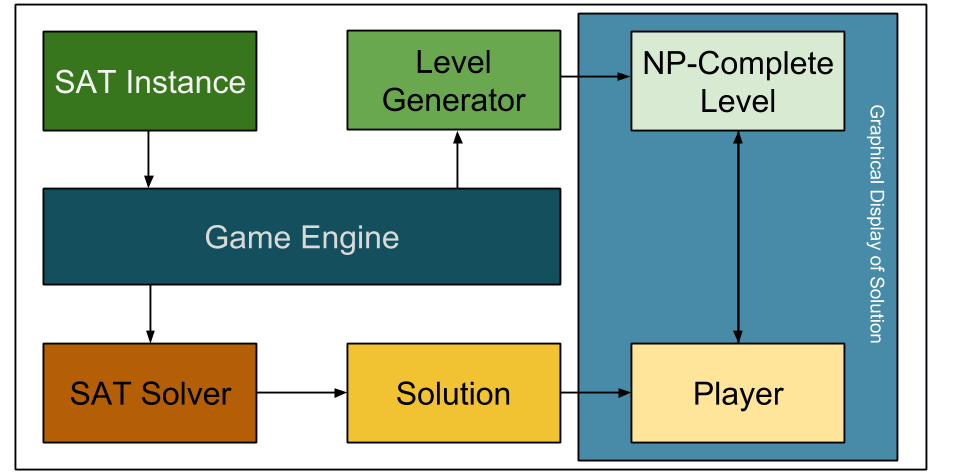
\includegraphics[scale=0.40]{modules2}
  \caption{Diagram demonstrating how the game engine modules integrate with one another to generate the level instance and provide the mechanism to provide a graphical solution.}
  \label{modules}
\end{figure}

The modules are designed to be as de-coupled and independent as possible, so as
to allow for greater independent development and more effective debugging.

% The Game State Manager class has a private
% member called \texttt{SAT\textunderscore Manager\textunderscore} which
% integrates the zchaff SAT solver into the game engine.


% \subsection{Reading in the CNF file}

% \subsection{Accessing variables and clauses}

% \section{Project wiki and references}

% A project wiki has acted as a journal and reference guide for the game engine's
% development. The rationale behind keeping this documentation was to allow for
% future development work to be carried out on the game engine.

% \section{Unit testing}

% The game engine source code also includes a testing framework for the various
% modules. In this project, googletest, Google's C++ Testing Framework was used.


\section{Game engine mechanics}


\subsection{Game loop and updating the game}

A \textit{game loop} provides the basic structure to implement a graphical game
as it provides the ability to update the sub-systems of the game and render
those changes to the screen \cite{Gregory:2009, Haller:2013:SGD:2556030}. The
loop is updated with a change of time since the last event (signified as the
variable \texttt{delta\textunderscore time}). As the game engine will
incorporate player AI, which will force the player sprite to solve the level, it
is necessary that the movement and rate of change is uniform.

This uniformity of change is achieved by creating a fixed
\texttt{delta\textunderscore time} value through creating fixed time steps.
Variable time steps would be more appropriate in game loops that have a wider
diversity of game object's updating \cite{Gregory:2009}.

The sprite and map classes are designed as tree structures that can be extended
to have child nodes pertaining to their particular class. This design, adapted
from \cite{Haller:2013:SGD:2556030}, allows for the game to be extended to
incorporate more features. The SceneNode class is extended into game entities
and objects. The inheritance allows for specialising certain class types while
retaining the core functionality and integrity of fixed time step in the game
engine design. These nodes are initialised and added upon the level
generation. This is explained in further detail in Chapter LEVEL GENERATION.


\subsection{Game states}

The game engine operates on game states. These states are kept by the
\texttt{game\textunderscore state\textunderscore manager} class in a private
\texttt{state\textunderscore stack\textunderscore}. Upon intialisation of the
game engine, the GSM registers and populates the stack. The game engine has distinct states:

\begin{itemize}
\item menu staet
\item instance selection
\item game state
\item pause state
\end{itemize}

In order to change the state, the current state requests to be `popped' (i.e.
removed) from the stack and `push' (i.e. add) the next desired state.

\subsubsection{Changing states}

The game engine states with the menu state. The menu state contains a select
instance option, a input option and an exit option. The first option takes the
user to a screen that has four arbitrary instances to demonstrate the game
engine's capabilities. The first is a single variable, the second is two
variables in two clauses. The third is a 3SAT instance and the 4th instance is
ten variables in ten clauses.

The pause state can be activated during the game \textunderscore state as well
as resume the game state.

\subsection{Managing input}

The input to the game is managed by the \texttt{player\textunderscore manager}
class. The input relies on assigning directional movement to the \texttt{mario}
sprite class. The \texttt{player\textunderscore manager} has a private
associative map, \texttt{action\textunderscore binding} which has
predefined movement values. This is made extensible for human input by being
able to be assigned to the keyboard via the \texttt{key\textunderscore
binding} member of the class.

The \texttt{player\textunderscore manager} pushes these action bindings into the
\texttt{comamand\textunderscore queue} object which is then 

This percise mechanism of selecting the appropriate path is detailed in Chapter
X, TITLE.

\subsection{Displaying to screen}

The \texttt{level} class contains the mario node, the mapnode and could be
extended to have a world object node.  Scene nodes are tree structures that draw
and interact.

The node receives a delta\textunderscore time variable which is the change in
time from the last update.

This is given to the scene node and any objects that have updated will. 

SFML provides for vertical synchronisation, which sets the call rate to the
display function in the library to be that of the monitors refresh rate. In this
way, the display of artefacts such as `screen-tearing', wherein the display
shows the information of two frames at the same time
\cite{Haller:2013:SGD:2556030}.

\subsection{Miscellaneous functionality}

\subsubsection{Mini-map}

The game engine display also includes a miniature map that contains the whole
level. This allows the viewer to see the scale of the level without

\subsubsection{Zoom}

\subsubsection{User input}

This is further detailed in the Evaluation chapter.

% \subsection{Player movement}

% \section{Drawing the tile}

% The levels are drawn using a tile-based method. There are a number of methods
% that could be used

\section{Chapter summary}

The game engine's design considerations and specifications have been grounded in
the concepts of re-usability and extensibility of the produced code in mind. The
core of the engine provides the necessary mechanisms for being able to generate
levels and display the solution, which will be covered in the next chapters..


%-------------------------------------------------------------------------------
% LEVEL GENERATION
%-------------------------------------------------------------------------------

\chapter{Level generation}

\epigraph{``Human beings are never more ingenious than in the invention of
games.''}{Gottfried Wilhelm Leibniz}

\section{Overview and specification}

One of the core featues of the game engine and stated research project goals is
to be able to generate game levels based on an arbitrary SAT instance. As
mentioned in the previous chapter, within the research project's game engine, a
`level' is a problem instance for the SAT solver to assess if there is a
satisfying assignment \cite{Aloupis2012} .

\section{The fundamentals of content generation}

In order to be able to generate game elements, the project utilises
\textit{procedural content generation} (PCG), which refers to automating the
creation of content for a game through the use of an algorithm
\cite{Hendrikx:2013:PCG:2422956.2422957, 5756645}. In this context, \textit{game
content} refers to all game elements, including the translated SAT gadgets,
excluding the player's own actions and the game engine \cite{Burgun:2012}. In
the game engine, this means

\begin{itemize}
\item level layout
\item generation of interactable objects
\end{itemize}

\subsection{Fundamentals of procedural content generation}

Content generation in video games combines a broad range of dynamic subject
areas including graphics, image processing, mathematics, artificial
intelligence, and ludology \cite{Hendrikx:2013:PCG:2422956.2422957}. PCG is
increasingly popular with recent titles employing elements of PCG to varying
degrees. This is due to being able to reduce the prohibitive expense of manually
creating game content \cite{Hendrikx:2013:PCG:2422956.2422957} and the ability
to generate new types of games based around content- generation \cite{5756645}.
From a game player perspective, a game that has infinite levels has greater
potential replay value, especially if the game adapts to the player's playing
style \cite{6424299}.

There are other, more practical reasons such as memory
consumption. The content. This has been used to tremendous effect in \textit{.kkrieger}, a
first-person shooter game, whose executable was a mere 95 KiB
\cite{Hendrikx:2013:PCG:2422956.2422957}.

For the purposes of the project, PCG allows for the ability to modify the level
instance, complete with the requisite gadgets, based on an arbitrary instance of
a SAT problem. This would remove the need to explicitly specify the game content
and could rely on algorithmic generation based on defined rules and limitations.

\section{Taxonomy of game elements and SAT instance gadgets}

This section provides an overview of broad definitions which will be used to
characterise the game engine's level generation mechanism.

\subsubsection{Online vs offline generation}

There is a distinction between \textit{Online content generation} occurs during
a video game's runtime. This is in contrast to \textit{offline content
generation} which is performed during the development of the game. The
requirements for effective online content generation are (i) that generation is
fast (ii) the content is reliable and correct \cite{5756645}.

\subsubsection{Necessary vs optional content}

Another set of distinctions is between \textit{necessary} and \textit{optional}
content. Necessary content is required for the progress and completion of the
game. Optional content is content with which the player may wish to engage but
does not prevent basic gameplay or completion of the game itself.

The importance is that necessary content must always be generated in a correct
manner. For example, a level must not be unsolvable nor should the game have an
undefeatable enemy, if such things prevent essential gameplay or render the game
impossible to complete.

\subsection{Requirements for Game Engine Level generation}

The project's game engine requires online content generation of necessary game
content. The elements need to be generated and are necessary for the successful
run of the game.

\subsection{Challenges in PCG}

Content generators can automatically create a large amount of differing levels
in a short amount of time but this is not a guarantee of the \textit{quality} of
the generated content \cite{Smith:2009:RLG:1536513.1536548}. Existing literature
regarding PCG identifies a lack of reliability and consistency in quality as a
main challenge area and barrier to wider adoption of PCG in commercial game
offerings. Zafar and Mujtaba \cite{6424299} assert that the majority of PCG
techniques are characterised by what they term \textit{catastrophic failures},
which make them unsuitable for wider commercial deployment. These failures
affect the reliability and accuracy of the game. The work identifies the
following as specific failures in 2D platform games:

\begin{itemize}

  \item height of ground;
  \item height of ground and optional content;
  \item simple level generation
  \item unplayable levels
  \item placement of the character's start position

\end{itemize}

\noindent The presence of these failures in the game engine would result in a
lack of communicability and visualisation of computational complexity. It is
therefore imperative that these failures be specifically guarded against and
tested for.

\subsubsection{Protecting against failure}

The generation algorithms may be tested through the use of \textit{fitness
functions}, which are objectively evaluates how closely a proposed solution
achieves a particular design aim. There is a question about which fitness
functions are useful and what sort of rules should be employed when generating
level. For example, Togelius \textit{et al}. \cite{togelius2007towards}
developed personalised fitness functions that would automatically generate
different racetracks based on the player's actions and skill.

\section{Content generation methodologies}

A number of approaches exist for content generation, of which X of the more
relevant were considered for level generation module of the game engine. Three
differing approaches will be surveyed and compared and evaluated for suitability
for use in the research project (see Figure~\ref{level}).

The simplest methodology is the constructive approach, wherein an algorithm
generates content based around a series operations that ensure that content is
produced according to the definitions of rules. In this way, the content
generated is `correct' insofar as adherence to the specified rules
\cite{browne2008automatic}. The algorithm does not test that the content has in
fact adhered to the rules however. While this method is restrictive, it has been
used to generate less vital game content such as terrain
\cite{Miller:1986:DRT:15886.15890}.

The other approach considered is `generate-and-test' approach. As suggested by
the name, there are two parts to this algorithm: After the content is generated,
it is then tested against constraints and assessed for compliance
\cite{5756645}. Content that does not pass assertion against these criteria is
discarded and is regenerated until it passes \cite{5756645}.

Search based generation is a specialised type of generate-and-test procedure.
Rather than merely accept or reject the generated content, the candidate content
is tested through a fitness function. The generation of new content is dependent
on the fitness value assigned to the prior evaluated instances. The goal is to
produce content that is qualitatively of increased value \cite{5756645}.



%%%%%%%%%%%%%%%%%%%%%%%%%
% The test function does not simply accept or reject the can- didate content, but grades it using one
% or a vector of real numbers. Such a test function is variously called a fitness, evaluation, and
% utility function; here, we will use “evalu- ation function” and call the number or vector it assigns
% to the content the fitness or simply the value of the content. • Generating new candidate content is
% contingent upon the fitness value assigned to previously evaluated content in- stances; in this way
% the aim is to produce new content with higher value.


\begin{figure}[h!]

  \centering
    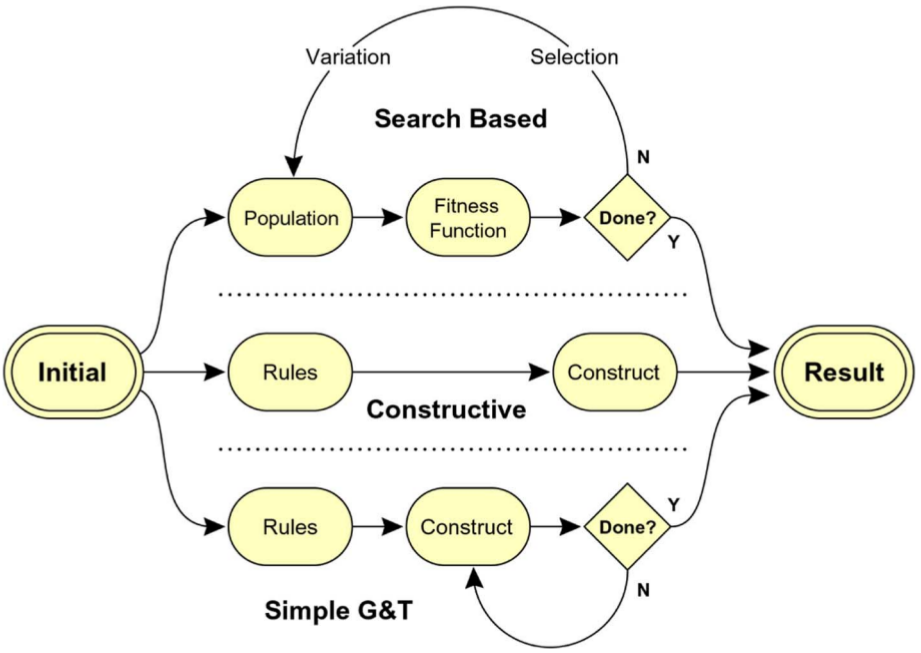
\includegraphics[scale=0.35]{lvlgenmethods}
  \caption{Representation of three types of level generation \cite{5756645}.}
  \label{level}
\end{figure}


\subsection{PCG heuristic techniques}

In each of the approaches above, there exits a difference between deterministic
and stochastic methods of generation. In the former, the generation tool will
generate specified content on each output. In a stochastic method, the results
are somewhat random.

Dormans and Bakkes \@\cite{dormans2011generating} presented a generative grammar
which allows for the generation of levels which are `correct' on a syntactic
level. This was achieved by dividing the content into mission and spaces. The
missions (or game tasks) are generated through the use of recursive, non-linear
graphs. From this output, the structure and shape of the level are constructed
from a separate `shape' grammar. The authors also utilised differing player
models in order to dynamically adjust difficulty, resulting in more adaptive
levels.


% To ensure efficient level generation, both Compton and Mateas
% \cite{compton2006procedural} and Smith \textit{et al}.
% \cite{Smith:2009:RLG:1536513.1536548} generate levels for 2D platform games by
% first splitting the levels into smaller sections. From a platform tileset, those
% smaller sections could be generated. This is the concept of `rhythm'-based
% generation: the pattern is derived from how the game is to be played. This
% allows for a range of the types of generated levels as well as maintaining the
% pacing of the game \cite{Smith:2009:RLG:1536513.1536548}. The
% Figure~\ref{level2} below illustrates the process.

% \begin{figure}[h!]

%   \centering     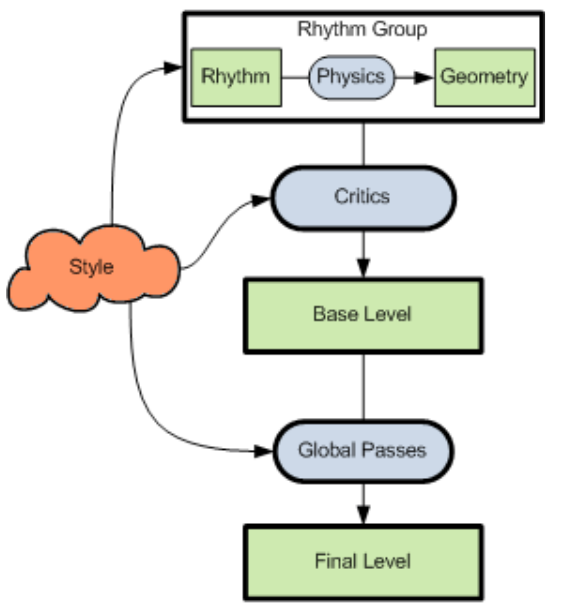
\includegraphics[scale=0.35]{lvlgen}      \caption{Level
% generation algorithm from \cite{Smith:2009:RLG:1536513.1536548}. The authors
% describe the green items as the generated content and blue boxes as constraints
% in order to ensure quality generation that adheres to specified criteria.}
% \label{level2} \end{figure}

% In a somewhat different fashion, the research from Jennings-Teats \textit{et
% al}. \cite{jennings2010polymorph} and Shaker \textit{et al}.
% \cite{shaker2010towards} demonstrate that a player's actions can be used for
% online generation of platform levels. This would entail that the game would
% model itself on the user's own style of playing. This is a more focused
% application of the approach used in Dormans' implementation
% \cite{dormans2010adventures}, which uses a pre-defined grammar to generate the
% mission structure. This is then implemented into the 2D-level using another
% grammar to translate this structure.

In a survey on the the evolution of game designs, Togelius and Schmidhuber
\cite{5035629} posit that `fun' in a game is derived from learning how to play
and ultimately mastering the mechanics. While this may be true to an extent
\cite{Burgun:2012}, the declaration and incorporation of these constraints into
an algorithm for generation is limited insofar as the design matches human
experience \cite{sorenson2011generic}.



% \section{Chapter summary}

% Level generation is a dynamic, growing area of video games research. There exist
% a number of different methodologies and approaches appropriate for the stated
% goals of the research project. For the purposes of the research project, many of
% these approaches are not necessarily applicable in initial design and
% implementation. Many studies, such as \cite{sorenson2011generic},
% \cite{5035629}, and \cite{smith2011tanagra} focus on creating varied content
% that is focused on player experience. This may not be an immediate priority in
% the research project as the focus is to be able to generate large levels that
% correctly represent SAT expressions.

% To this end, the rhythm-based approach
% \cite{compton2006procedural,Smith:2009:RLG:1536513.1536548} and `chunk approach'
% \cite{mawhorter2010procedural} are most pertinent as it would allow various
% gadget clauses to be pre-created and joined together to make larger scale levels
% to be solved. The creation of an efficient algorithm (even a genetic one
% \cite{mourato2011automatic}) represents an area of future research. This will be
% further explored in the next chapter on design considerations.

% In the previous chapters, the basis for making a 2D platform game NP-hard was
% established. In this chapter, the focus will be on designing a playable level
% that incorporates those elements.

% In previous literature, the level design has focused on the gadgets that
% correspond to 3SAT reductions in order to prove that the game is in fact NP-
% hard. In these models, the actual gameplay is generalised and left-otherwise
% unaddressed.

% This provides a challenge when

\section{Designing NP-complete levels}

% Review Aloupis and Forisek and others

\subsubsection{Implementing the frameworks established in literature}

The level design implemented in the project uses the model in Aloupis \textit{et
al}. For the purposes of this project, the size of the levels are $n\times n$ ,
which means that the size is essentially unlimited.



% \section{Modifying the model in 

% The Aloupis et al model

% \subsection{Modification 1: Joining the variable with the clause}

% In the A model, the player assigns a value to variable by deciding to fall down
% one side or another. The fall leads to a clause where that literal resides. The
% player then renders the clause TRUE by performing the action. In reality, it
% does not matter whether the

% \subsection{Modification 2: Progressing to the next variable assignment}

% This issue was addressed by utilising the warp pipes in \textit{Super Mario
% Bros.} In the game, the player can make use of certain pipes to travel either to
% different areas  of the level that would otherwise not be accessible or to other
% levels entirely.

% The use of warp tunnels has two functions: (1) it allows for a neat way in which
% to demonstrate clauses

% In the Aloupis model, the need for enemies does not feature as prominently as
% with  Forisek. Forisek contends that enemies are required in order to

% \subsection{Modification 3: Preventing cross-over}

Figure~\ref{full-level} demonstrates how the gadgets may be phsyically linked
together in a three variable, three clause 3SAT reducation.

\begin{figure}[ht!]

  \centering
    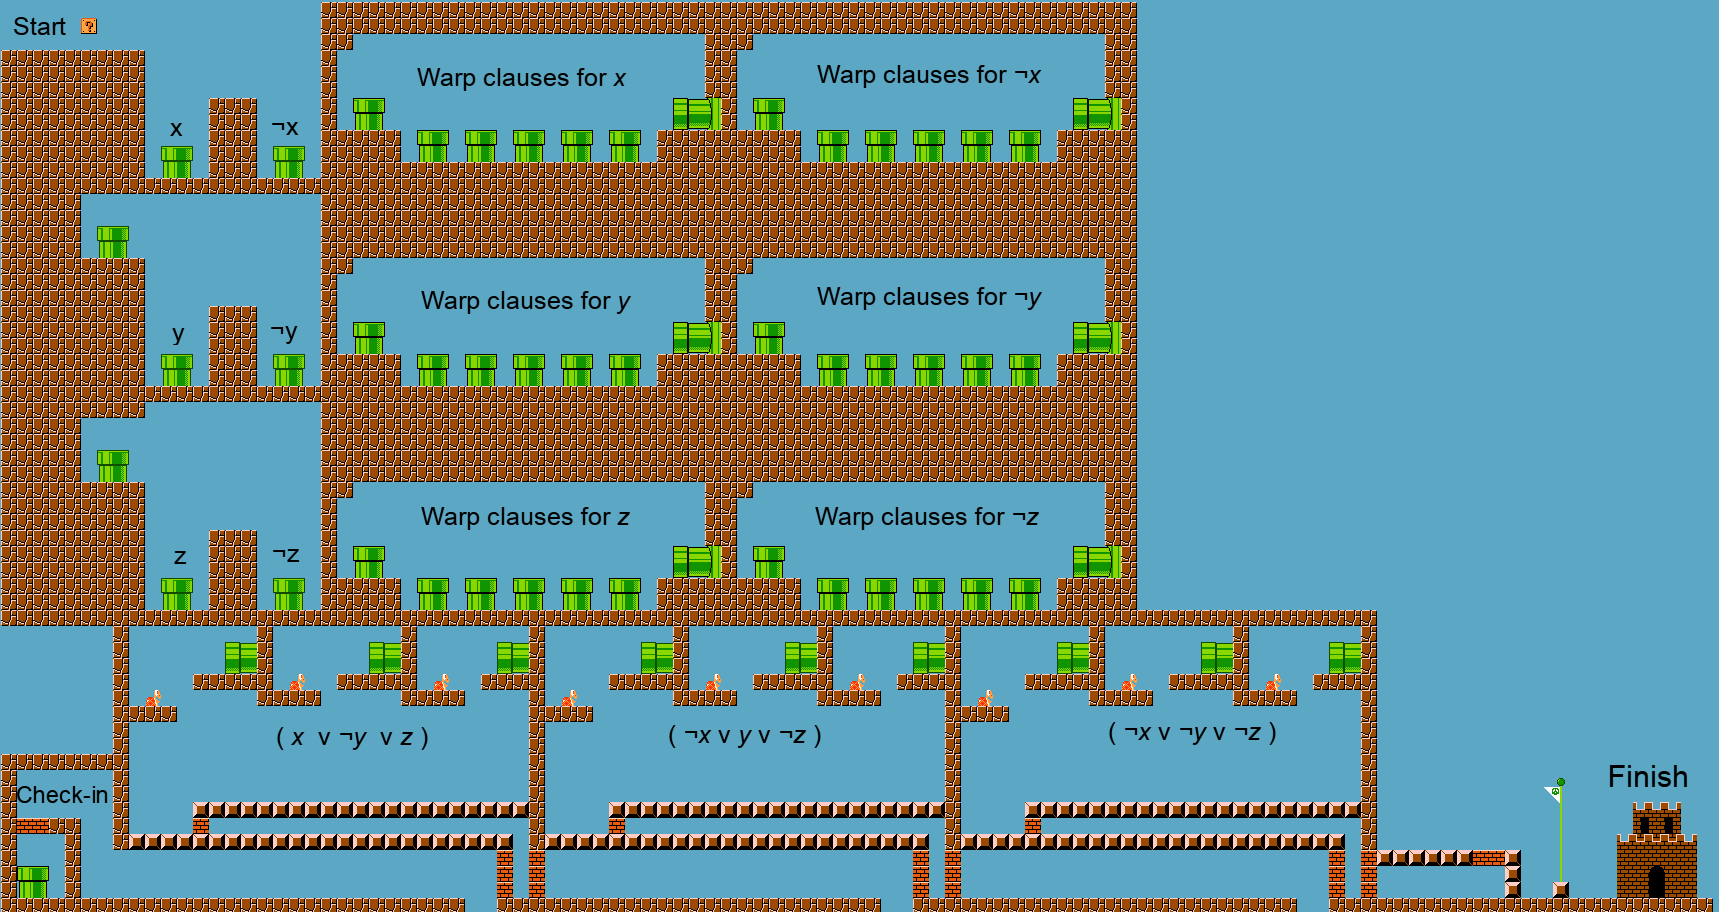
\includegraphics[scale=0.26]{basic_level}
  \caption{Representation of physical linking of gadgets.}
  \label{full-level}
\end{figure}

This will be briefly described below.

The player starts as in the framework described by Aloupis \textit{et
al}\cite{Aloupis2012} with a start gadget. In the current game engine, there is
no necessity to have an animation that turns `small' Mario (composed of a single 16x16 tile) into Super
Mario. Super Mario can jump under bricks and break certain types of blocks. 

% Cross over gadgets

The variable gadget relies on the meta-theorem provided by Fori\v{s}ek
\cite{DBLP:conf/fun/Forisek10} (long fall). In Aloupis et al \cite{Aloupis2012},
the authors created a cross-over gadget that prevented the player from by-
passing or accessing areas of the level which impact the reducation to a 3SAT
instance. The authors are not clear exactly how the gadgets are physically
linked together in order to create a complete functioning level. In particular,
the  This presentes a number of challenges when scaling a level. In Aloupis, the
3SAT instance has three clauses. However, when dealing the amount of cross-over
instances increases.

In order to efficiently

In \textit{Super Mario Bros.}, the player may discover that certain pipes are
able to be utilised in order to travel to different hidden areas or even other
levels. This game mechanic provides an immediate solution to scalability for the
purposes of the project's development.

In the project's implementation, after the player picks a variable by falling
and using the pipe, the player is taken to a clause choosing gadget. Here there
are a series of pipes, each leading to a particular clause where the literal
appears.

\begin{figure}[ht!]

  \centering
    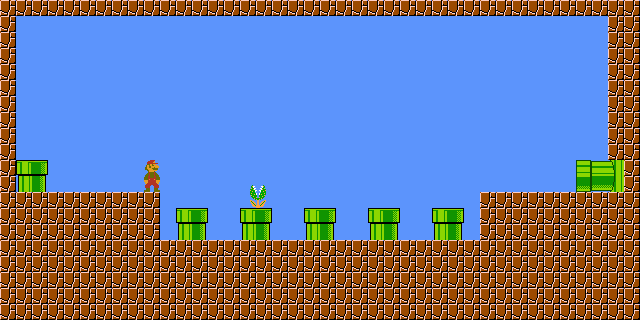
\includegraphics[scale=0.70]{clause}
    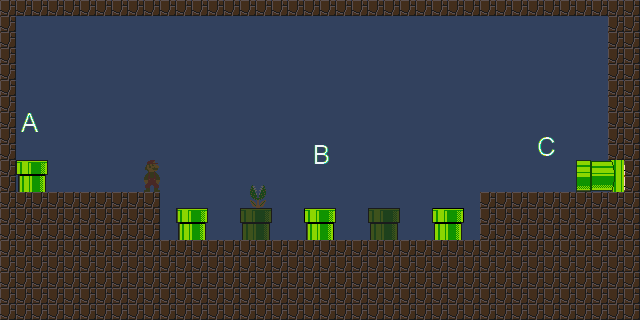
\includegraphics[scale=0.70]{clause-explain}
  \caption{Crossing into other clause areas.}
  \label{clause-crossing}
\end{figure}

% \begin{figure}[ht!]

%   \centering
%     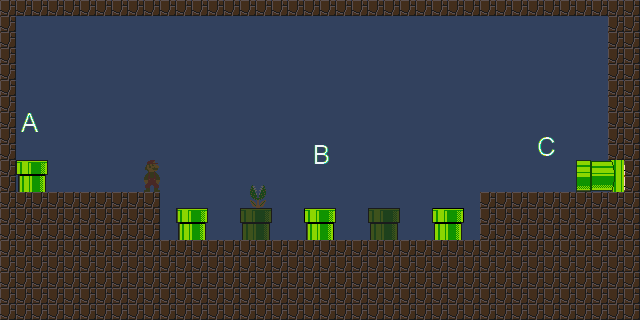
\includegraphics[scale=0.70]{clause-explain}
%   \caption{Crossing into other clause areas.}
%   \label{clause-crossing-explain}
% \end{figure}

In the clause-crossing gadget, the player enters on the pipe on the left (marked
A). The player is not able to return through this pipe. Even if it was the case,
the player cannot overcome the variable gadget.

There are five pipes of which three lead to clauses and the other two contain
\textit{Piranha plants}, venus-fly trap like enemies in \textit{Super Mario
Bros} (Marked B). Once the clauses have been visited and unlocked, the player
returns through the pipe on the right side of the screen (marked C) and can
proceed to the next variable assignment. If the player has no more variable
assignments to make, the pipe will lead to the check-in gadget, illustrated in
Figure~\ref{check-in}. The check-in gadget allows the player to progress through
the check-out and ultimately to the finish gadget.

\begin{figure}[ht!]

  \centering
    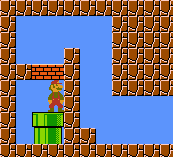
\includegraphics[scale=1.2]{check-out}
  \caption{The check-in gadget. Note the player can only advance as Super Mario.}
  \label{check-in}
\end{figure}

Once the player checks-in, the player then advances through the check-out of the
level. The check-out phase is only passable if the clauses have been opened. The
only obstacle at this point of the game is the drop in the floor. The player
then proceeds to the finish gadget, shown in Figure~\ref{finish}.

\begin{figure}[ht!]

  \centering
    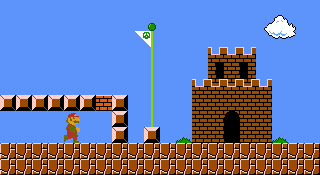
\includegraphics[scale=1.0]{finish}
  \caption{The check-in gadget. Note the player can only advance as Super Mario.}
  \label{finish}
\end{figure}

\section{Chapter Summary}

There exist innumerable means of achieving online generation for necessary game
elements. In this project the approach has been to utilise a generate-and-test
methodology for the game elements. 7

%-------------------------------------------------------------------------------
% PLAYER SOLVING
%-------------------------------------------------------------------------------

\chapter{Player AI}

\epigraph{``It's not hard to make decisions when you know what your values
are.''}{Roy Disney}

\section{Overview}

Having established the procedural generation of the game level based on the SAT
instance in the previous chapter, this chapter focuses on the game engine's
player AI. The player AI directs and controls the player sprite's movement and
path selection, which corresponds to the solution to a SAT instance.

\section{Identifying the appropriate path}

As descibed in the above section (SOME SECTION) in Chapter (Game Design), the
movement of the player sprite is controlled and regulated by the player-manager
class. To briefly summarise, the player-manager class sends a queue of commands
(via the command-queue object) to the level class, where the movements are
rendered to the screen. 

\subsection{Receiving SAT instance values}

After the initialisation of the game-state, the level class loads the zchaff
manager nad the variable manager, solving the arbitrary SAT instance.

If the ENTER button is pressed, these objects are set as values within the
player-manager, in order for the

The player-class has a var-manager member. 

\subsection{Generating commands}

The player AI relies on \texttt{command} objects which, when executed, move the
player sprite to the appropriate location and identify to both the level
instance and the player manager which gadget is being solved and where the
location is provided. This section provides an indepth look into the mechanics
of commands and how these are generated within the player-manager.

\subsubsection{Overview of command structures}

A command is a data structure comprised of a \texttt{Location}, an enumeration
of game gadgets, and an \texttt{Action}. The \texttt{Action} is a type alias for
a class template for a polymorphic function wrapper for a lambda expression.
This is provided in the C++11 standard. \texttt{Action} takes a
\texttt{SceneNode} and \texttt{delta\textunderscore time} as arguments. These
are downcast in some manner that needs explaining.

SFML BOOK NEEDED

\subsubsection{The available actions}

The actions that are available to the player-manager to move the sprite in the
appropriate direction are: 
\begin{itemize} 
  \item MoveRight 
  \item MoveLeft 
  \item Down 
  \item Jump 
  \item Wait
\end{itemize}

As mentioned in the previous chapter, the level instance is generated on a
$16\times 16$ tile world. The MoveRight and MoveLeft movements move 2.f or 1/8th
of a tile space per movement. The Down movement represents a fall and consists
of 16.f (e.g. a whole tile). Similarly, the Jump action displaces the player-
sprite a whole tile as well. This means that the sprite's jump is exactly twice
its height. This is in keeping with the meta-theorem of characteristics of 2D
platform video games that are NP-complete.

\subsubsection{Identifying the correct clause location}

The display of the solution requires that the assigned variable satisfy the
appropriate clause when it evaluates to true in that clause. The player sprite
should not warp to those clause gadgets where the variable assignment does not
render the clause true. In order to achieve this, the player-manager sets the
appropriate location of each assigned variable prior to providing the requisite
commands.

Once the solution display has been initiated, the level instance passes a
pointer to its command-queue member to the player-manager through its public
\texttt{SetSolutionQueue} member function. Within this function, the player-
manager initialises its assigned-variables- member, which sets the assignment
solution and passes this to the 
\par \noindent \texttt{SetAssignmentLocation} member function.
Here the player-manager iterates through the clauses and where the current
variable being assigned matches one in the clause, this is pushed onto the
location-map.

The location-map is a 2D vector structure. Each row corresponds to the variable.
Each column in that row contains a value which corresponds to the clause which
contains that assigned variable.

\subsubsection{Providing the requiste information to each command}

The player-manager class has a number of member functions that have pre-defined
movement elements to traverse each type of game gadget. The pre-defined elements
concern length of walk, jumps, falls and waits. These are then added in a 
for-loop with the necessary information about location, current variable, current
clause, and whether there is an animated action sequence involved.
\begin{lstlisting}
  // Move the sprite right
  for (int i = 0; i < 8; ++i) {
    Command c         = action_binding_[MoveRight];
    c.location_       = c.Clause;
    c.var_assignment_ = current_variable_;
    c.current_clause_ = target_clause;
    c.has_action_     = false;
    commands.Push(c);
  }
\end{lstlisting}

After the location-map has been generated, the command-queue is passed to
\texttt{InitStartQueue}, which provides the start sequence. This then passes the
command-queue to the Warp Gadget, then to the Clause gadget. If there are no
clauses left, the player-sprite proceeds to the warp exit and to the next
variable. The process starts again.

Where there are no more variables to solve, the warp exit will take the player-
sprite to the checkin gadget, where the checkout process commences. After
clearing the checkout, the player proceeds to the finish gadget and the instance
is solved.

\subsubsection{Making an assignment decision}

The gadgets in the game require a decision to be made regarding the assignment
of variables. This means that the player-sprite may choose left for a TRUE
assignment or right for a FALSE assignment. This is achieved by assessing the
current-variable member and initiated the correct sequence which has been
predefined.


\subsection{Positioning the sprite in the level}

Having established the correct commands for the appropriate game gadgets, the
player-manager class returns the command-queue to the level instance.The level
instance will take current command and, depending on the Location enumeration,
positions the sprite in the appropriate position as well as trigger and world
object events.

The positioning of the player sprite is achieved through its update

\subsubsection{Travelling between the warp and the clause gadgets}

The player-sprite has a location member variable that is updated upon every
move. Where the command requires that the player warp to the clause gadget, the
level instance keeps the location prior to the warp. The player-sprite is then
warped to the clause gadget and the actions are performed there. Once that
action is performed the player return through the pipe and is re-assigned the
prior jump position, ensuring that the player-sprite is returned appropriately
and the game actions adhere to the game mechanics and logic.

\section{Chapter summary}

The player AI utilise the SAT instance's specifics as well as the definitions of
the variable gadgets in order to determine the appropriate course of action.
This is achieved through the command structure which passes the necessary
information between the level instance and the player-manager class.

% ------------------------------------------------------------------------------
% ANALYSIS
% ------------------------------------------------------------------------------

\chapter{Implementation and evaluation}

\epigraph{`` One of the great mistakes is to judge policies and programs by
their intentions rather than their results''}{Milton Friedman}

To this point, the discussion has focused on the theoretical background of
computational complexity of video game, followed by the design considerations
and model of the game engine.  This chapter therefore provides analysis of the
analysis of the functionality of the developed game engine and
evaluates the results against the project's success criteria.

\section{Establishing assessment criteria}

Within a project that is strongly focused on implementation, the assessment of
whether the development has been successful lay within the domain of software
evaluation methodology. To this end, there exist a number of evaluation
methodologies for software development \cite{unterkalmsteiner2012evaluation}.
These range from a series of tests to examine the qualitative merit of
functionality and ability to meet specification.

The assessment methodology employed in this project has been to determine
whether the software produced met its original goals. These goals have been
consistently reiterated since the inception of the project and formalised as the
design specification.

\subsection{Evaluation criteria for this project}

At the start of the project's development cycle, an evaluation criteria was
developed in order to track as objectively as possible whether the project had
met its goals. This had been established prior to any code being written as it
objectively signalled when progress had or had not been made.

The success of the project is comprised of the following elements:

\begin{itemize}
\item the game engine should be able to take an arbitrary SAT instance and 
transform it into a video game level modelled on a framework establishing the 
NP-completeness of a 2D platform video game;
\item the game engine should incorporate a SAT solver in order to solve the SAT instance;
\item if a satisfying assignment to the instance exists, then the player AI should
identify the correct path to solve the level. 
\item the game engine should not experience catastrophic failures in its content generation
\item the game engine should be extensible and adaptable to other SAT instances and complexity classes.
\end{itemize}


\section{Generating a graphical solution display}

After the initial game loop and drawing mechanisms were achieved, the project's
attention turned to SAT solver integration and graphical display. To examine
differing approaches, prototypes were devised and tested. In the Graphical SAT
experiment, a simplified game loop was developed. 

The zChaff library was then linked to the game loop and variable objects were
created. The variable object class contained a shape and an assignment value.
The zchaff manager class would have a sequence container (i.e.
\texttt{std::vector}) which would load the variable objects in the manner in
which they appeared in the formula. 

The game engine would then step through each assignment and change the colours
of the gray circles to green (for TRUE) or red (for FALSE). When a clause was
satisfied, the grey circle near the clause would light up green. Once all
clauses evaluated to true, the game engine would declare the formula satisfiable
on screen, as illustrated in Figure~\ref{graphicalSAT} below.

\begin{figure}[ht!]

  \centering     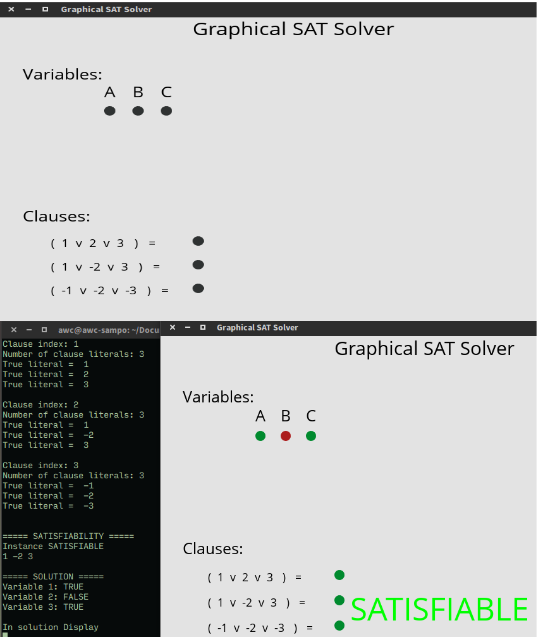
\includegraphics[scale=0.4]{graphicalSAT}   \caption{An
experiment in displaying the satisfiabilty solution to a SAT instance. The top
screenshot illustrates the unassigned variables within the formula towards the
top and the clause representations on the bottom. The bottom screenshot shows
the correct assignment in the terminal and the corresponding graphical
representation.}   \label{graphicalSAT} \end{figure}

\subsection{Graphical SAT experimental outcomes}

This experiment had implications for both the level generation and the player
AI. The level generation module benefitted from understanding how the zchaff
manager could be extended to read in the correct values and store these in what
would become the variable-manager. Work from this point went on to the MapChunk
and MapChunkManager classes (described in the next section).

\subsubsection{Non-scalability of drawing methodology}

The display is drawn to the screen in a sequential manner through a simple do-
while loop. This drawing implementation was appropriate for this rudimentary,
experimental prototype, but was identified as not being scalable to the game
engine. This is because the do-while loop requires constant calls to the draw()
function which intereferes with the game loop design and fixed time steps (see
Chapter X).

\section{Level generation verification and testing}

Having successfully been able to sequence the satisfying assignment and display
to screen, the next development focus was the MapChunk and the MapChunkManager.
The specifics of these classes and their functionality are detailed in Chpater
LEVEL GENERATION.

To test and assert that the specific map chunks were (a) being correcty loaded
and (b) correctly called, were tested in the MapChunkTest.cpp file. The test
loads mapchunk strings into a 2D vector. These are then tested against those
read into game engine. 

The test checks if there is an equality of values in the test vectors and those
of the game engine. If the so, the value should return true. If such equivalence
is not present or there is an error, the returned value should be false.

This form of testing allowed for the verification that the MapChunkManager was
correctly perfoming its role and allowed for further implmentation in level
generation and player AI development.

//////SOME KIND OF GRAPHIC /////

\section{Graphical element positioning and offsets}

A consistent challenge in the implementation of the game engine software was
managing the positioning off sets in an extendable and flexible level
generation. Where a world object (e.g. koopa shell, brick, or flag) needed to be drawn

The tests for this occurance where assertions within the code (i.e. expecting
certain elements to be drawn in certain places) and visual inspection. As
mentioned in previous sections, positions of objects are provided in as float
values in SFML so as to provide precision. However, the pixels are drawn in
integer values. The rounding of the values is done internally within SFML, so if
certain offsets are desired, these have to be provided before being drawn to
screen.

\section{Verification of formula satisfiability}

One of the most crucial features of the. To achieve this, the satifying
assignement of the formula is provided by zchaff, this value is then checked
that it is consistent throughout the game engine and the output is able to be
visually inspected in the terminal.

\section{Animations}

Animations for the sprite and events had also been addressed during the
implementation and assessment of the game engine. The game engine includes
modest and simple animations in order to display in a more relatable manner to
audiences. This aspect of the game engine was considered a lower priority, as
animations and their implementation were not explicit research goals, being
incidental to the creation of a game engine. To this end, animations were
addressed insofar as being a means to faciliate visualisation.

The player sprite has a basic walk cycle that is composed of three frames. The
play in sequence when the moving left or moving right Boolean flags are set in
the Mario class. When there is no movement, the cycle resets to the standing
frame.

To move in the opposite direction, the frames are mirrored so that the sprite
now faces the opposite direction. This is beneficial in that 

During the development an Animation class was added, based on tutorial material
available \cite{Haller:2013:SGD:2556030}. This could allow for further
extensibility by adding more animated Koopas or other eneimies. 


\section{Implementation analysis summary}

As with any software implementation, the game engine development was beset by
challenges which spanned trivial to fundamental in nature. This chapter serves
as a highlight of the most significant milestones and issues that characterised
the development of the implemetnation. The nature and evaluation of the
obstacles and problems challenging the success of the project are further
elaborated upon in the following chapter.

% ------------------------------------------------------------------------------
% EVALUATION
% ------------------------------------------------------------------------------

% \chapter{Evaluation}

% \epigraph{``QUOTE.''}{Someone}

% \section{Overview}

% This chapter examines and evaluates the implementation of the game engine
% software as well as explore alternative methodologies and approaches to the
% challenges that had been identified.

% \section{Evaluating implmentation and the challenges to implementation}

% There exist a number of evaluation methodologies for software development
% \cite{unterkalmsteiner2012evaluation}. These range from a series of tests to
% examine the qualitative merit of functionality and ability to meet
% specification. 

% \subsection{Evaluation criteria}
% The success of the project is comprised of the following elements:

% \begin{itemize}
% \item the game engine should be able to take an arbitrary SAT instance and 
% transform it into a video game level modelled on a framework establishing the 
% NP-completeness of a 2D platform video game;
% \item the game engine should incorporate a SAT solver in order to solve the SAT instance;
% \item if a satisfying assignment to the instance exists, then the player AI should
% identify the correct path to solve the level. 
% \item the game engine should not experience catastrophic failures in its content generation
% \item the game engine should be extensible and adaptable to other SAT instances and complexity classes.
% \end{itemize}

% The following section will assess the extent the project has met its objectives.

\subsection{Assessment against evaluation criteria}




\begin{center}
\begin{tabular}{ |p{5.5cm}|p{3cm}|p{5.5cm}|  }
 \hline
 \multicolumn{3}{|c|}{Game Engine Evaluation} \\
 \hline
 Assessment Goal & Completed & Notes \\
 \hline
 Integrate suitable SAT solver  & Yes &   \\ \hline
 Create Game Loop with fixed time steps &   Yes  &    \\ \hline
 Successfully read in DIMACS CNF file format & Yes &  \\ \hline
 Generate NP-complete level based on SAT instance  & Yes & \\ \hline
 Solve NP-complete level with adaptable player AI &   Yes &   \\ \hline
 Identify the location of literals within clauses for AI & Yes  &    \\ \hline
 Capture user input for arbitrary SAT instnace & AO  & AGO \\ \hline
\end{tabular}
\end{center}


\subsection{Identifying solutions}

\section{Alternative approaches to content generation and player AI}

As with any software development cycle, a number of alternatives to the selected
methodology are available and may have been better.

\subsection{Using Binary Decision Diagrams}

The project's implementation has relied on a SAT solver in order to provide a
solution to the SAT instance. However, this is not the only means by which to
solve the instance. Binary decision diagrams are data structures that represent
Boolean functions.

/////wiki ///

s a data structure that is used to represent a Boolean function. On a more abstract level, BDDs can be considered as a compressed representation of sets or relations. 

///

This could be an alternative means upon which to base the player AI. Howver, there do exist certain issues. The use of BDDs is somewhat limited as the size of at run-time may increase a lot. 

///// Unfortunately, their use is
rather limited due to the size explosion problem. It has been
observed that so long as the BDD size can be contained, solutions
can be found quickly, often with predictable run-times
[6] [7] [23].
////


In literature, a SAT solver may be used or a BDD but not both. However, there
are efforts to combine the two.

\subsection{Alternative procedural content generation approaches}

The approach taken in this

Establishing a scripting language would provide even further granularity. 

Sorenson \textit{et al.} \@\cite{sorenson2011generic} proposed that content
generation should  levels that is founded on an explicit model of the
relationship between challenge and fun. The author wanted to increase the fun
level of player and the challenges should not bore the human. Therefore he
modelled a fitness function and levels were designed for \textit{Super Mario
Bros} with high accuracy. The technique insures that human will generate certain
portion by hand and then the model used will evaluate the content generated –
this evaluation is similar to the evaluation of automatic content. The levels
will be a mixture of straightforward and difficult portion like the rhythm-group
structure of high and low nodes, giving games more interesting levels.

Mourato \textit{et al.} \cite{mourato2011automatic} proposed using a genetic
algorithm in order to generate game content for human-players. A genetic
algorithm is a search heuristic that generates approximations through selection
and mutation \cite{srinivas1994genetic}. The authors achieved modest but
positive results including increased level variety and ability to add necessary
and optional content correctly. This method is not entirely suitable for the
current research project as the authors' goals has been to

Smith \textit{et al.} \@\cite{smith2011tanagra} presented a design tool
(TANAGRA) that merged the input from the game designer and the PCG algorithm to
produce levels for a 2D platform game. The technique allowed the designer to
establishes rules and constraints to specify specific content, but allows the
algorithm to decide that which is unspecified. The authors content that this
provides for more diversity in level design as well as enhanced entertainment
value.

A rhythm-based technique is common approach to automatic level generation.
Mawhorter and Mateas \cite{mawhorter2010procedural} devised the `occupancy
regulated extension' algorithm which stitches together samples (referred to
`chunks') authored by human developers into a playable level. This method
described here could be combined with. This is further elaborated upon in the
next chapter on design considerations.

% \section{Use of C++}

% The use of C++ as the development language is good. There are others but C++
% allows for scalability.

% There is scope for procedurally generating content using other languages. One
% explored was Haskell.

% \section{Use of Haskell to generate content}

% ------------------------------------------------------------------------------
% FUTURE WORK
% ------------------------------------------------------------------------------

% \chapter{Future Work}

% \section{Constrained level size}

% As mentioned in Chapter X, the  level that is 14 x 14 tiles as the original SMB was.

% \section{Additional complexity classes}

% \subsubsection{PSPACE}

% \subsubsection{EXSPACE}

% \section{Web Deployment}



% ------------------------------------------------------------------------------
% CHP 6 --- SUMMARY AND CONCLUSIONS
% ------------------------------------------------------------------------------

\chapter{Conclusions and future work}

\epigraph{``QUOTE.''}{Someone}

\section{Overview}

% The research review has established a broad theoretical basis from which to
% begin the modelling developing a viable design of the game engine, as
% illustrated in the previous chapter. As a consequence, the implementation and
% development of the game engine design will now be able begin its preliminary
% stages. To this end, the outcome of the research review has been successful and
% its scope complete.

% This however does not mean that the review of literature has been completed for
% the entirety of the research project. The current review will continue to be
% augmented and developed in parallel with the development of the game engine
% software implementation. Already this review has identified new areas of
% investigation in order to complete the research aims of the project. This is
% contained in the future work section below.

\section{Future work}

% \subsubsection{Selection of appropriate SAT features}

% During the implementation, further review and investigation will be conducted
% into the heuristic selection features of SAT solvers. This will be done in order
% to select appropriate solvers which can efficiently interface with the software
% in order to provide for successful visualisation of complexity problems.

% \subsubsection{Ability to run multiple SAT solvers simultaneously}

% An idea that had surfaced was the concept of being able to run two different SAT
% solvers (e.g. zChaff and MiniSAT) simultaneously during a problem instance. The
% literature was not clear on the subject and as such requires further
% investigation and experiment to evaluate whether this could constitute a feature
% of the game engine.

% \subsubsection{Experiments with level generation}

% A greater investigation will be needed once the content generation techniques
% are developed and utilised. At this the current stage, it is not possible to
% know what sort of challenges may arise during implementation, as research has
% been solely based on heuristic models.

% \subsubsection{Identification of further complexity classes}

% After the successful integration of software features, the literature review
% will benefit from identifying other possible classes of complexity that could be
% tested within the developed software.


% ------------------------------------------------------------------------------
% BIBLIOGRAPHY
% ------------------------------------------------------------------------------

\bibliographystyle{abbrv}
\bibliography{references.bib}
\end{document}
